\documentclass[12pt]{article}
\usepackage[
    top=10mm,
    bottom=10mm,
    left=10mm,
    right=10mm,
    marginparwidth=0mm,
    marginparsep=0mm,
    % headheight=15pt,
    centering,
    % showframe,
    includefoot,
    % includehead
]{geometry}

\usepackage{tikz}
\usepackage{tikz-cd}
\usepackage{multicol}
\usepackage{hyperref}
\usepackage{breqn}

\usetikzlibrary{shapes.geometric}

\hypersetup{
    colorlinks=false,
    linktoc=all,
}

\renewcommand{\date}[1]{\underline{\bf #1}}

\def\eps{\varepsilon}
\def\range{\text{Range}}
\def\proj{\text{proj}}

\newcommand{\GCD}{\text{GCD}}
\def\RowSpace{\text{RowSpace}}
\def\ColSpace{\text{ColSpace}}
\def\trace{\text{trace}}
\def\Ann{\text{Ann}}
\def\sgn{\text{sgn}}
\def\B{\mathcal B}
\def\P{\mathcal P}
\newcommand{\lcm}{\text{lcm}}
% \newcommand{\Aut}{\text{Aut}}

\def\phi{\varphi}
\def\sgn{\text{sgn}}
\def\image{\text{image}}

\def\Tinv{$T$-invariant}


% create a command for TODOs
\newcommand{\TODO}{\color{red}\textbf{TODO}\color{black}}

\newcommand*{\xdash}[1][3em]{\color{darkgray}\rule[0.5ex]{#1}{0.55pt}\color{black}}

\newcommand{\ip}[2]{\left( #1 \mid #2 \right)}

\newcommand{\lr}[1]{\langle #1 \rangle}

% preamble
\input{preamble}



% colors used in proof boxes
\definecolor{proof_fg}{HTML}{ABABAB}
\definecolor{proof_bg}{HTML}{EDEDED}



% box solutions
\newenvironment{solution}{
  \begin{leftbar}

  \noin
  {\large \sc solution} \\
}
{

  \medskip
  \noin
  \textcolor{proof_fg}{$\blacksquare$}

  \end{leftbar}
}



% style a problem and solution
\newcommand{\prob}[3]{
  \bigskip \bigskip \noin
  {\Large\sc Problem #1}

  \medskip\noin
  #2

  \begin{solution}
    \noin
    #3
  \end{solution}
}

\renewcommand{\mod}[1]{
  \text{ (mod $#1$) }
}

\def\mat{\text{Mat}}
\def\gl{\text{GL}}
\def\sl{\text{SL}}



\begin{document}

\tableofcontents

\date{Wed. 24 Jan 2024}

\note {
All info for the class is available on the canvas page.
Notes from the prof are written on the iPad, and PDFs will be provided after
each class. Despite this taking notes is helpful.

Offices are hours are Tuesdays in person, and Thursdays on Zoom. Hours may
vary.

A text for this class is not {\it required}. Technically, we are using
Fraleigh's {\it A first course in Abstract Algebra}

No quizzes in this class, weekly Homeworks except on Exam weeks, two
midterms, and one final.

Readings on the class schedule are not additional, it's for people that need
extra material, or people that missed that day.
}

\section{Introduction - Sets and Relations}

\subsection{Sets}

\definition{
	A {\bf Set}. is a well-defined collection of objects called {\it elements}.

	$a \in A$ means ``$A$ is a set, $a$ is an element of a set, and $a$ is in
	$A$.
}

Examples of sets are

\begin{itemize}
	\item $\Z$ - The set of all integers, positive, negative, and zero
	\item $\N$ - The set of natural numbers, $0, 1, 2, \dots$. {\bf In this
			      class, $\N$ starts with $1$.}
	\item $\Q$ - The set of rational numbers.
	\item $\R$ - The set of real numbers.
	\item $\C$ - The set of complex numbers.
	\item $\{1, 2, 3, 4\}$
	\item $\{a \in \Z \mid a > 2 \}$. This is a set of integers {\it such that} $a
		      > 2$.
	\item $\varnothing$ - The empty set.
	\item $\text{GLn}(\R)$ - The set of $n \times n$ invertible matrices with real
	      entries. (GL stands for ``General Linear".)
	\item $C(\R)$ - The set of continuous functions $f: \R \to \R$.
\end{itemize}

\definition{
	A set $A$ is a {\bf subset} of a set $B$ if

	\[
		\forall x \in A, x \in B
	\]

	In other words, everything in $A$ is also in $B$. As notation, we can say
	either $A \subseteq B$ or $A \subset B$.

	A {\bf proper} subset is $A \subset B$ but $A \ne B$. Just write $A
		\subsetneq B$.
}

For example, $\N \subseteq \Z \subseteq \Q \subseteq \R \subseteq \C$. And,
importantly, $\varnothing \subseteq A$ for all sets $A$. In other words, the
empty set is a subset of {\it all} sets.

Two sets are equal if $A = B$, or $A \subseteq B$ {\it and} $B \subseteq A$.
This is often how you prove set equality.

\subsubsection{Set Operations}

We have four main operations.

\begin{itemize}
	\item {\bf Union}: $A \cup B = \{x \mid x \in A \text{ or } x \in B \}$.
	\item {\bf Intersection}: $A \cap B = \{ x \mid x \in A \text{ and } x \in B \}$.
	\item {\bf Product}: $A \times B = \{(a, b) \mid a \in A, b \in B \}$.
	\item {\bf Difference}: $A \setminus B = \{x \mid x \in A \text{ and } x \not\in B\}$
\end{itemize}

Two sets are {\bf disjoint} if $A \cap B = \varnothing$.

If we're working in a particular {\it universe} $U$ (i.e. all sets are subsets
of the universal set $U$) then the {\it complement} of $A$ is $A^c = \{x \mid x
	\in U \text{ and } x \not\in A \}$.

\subsection{Relations}

\definition {
	A {\bf relation} between sets $A$ and $B$ is a subset $R \subseteq A \times
		B$.
}

If $(a, b) \in R$, then we say that ``$a$ is related to $b$", or we write
$aRb$, or $a \sim b$.

\example {
	$R \subseteq \{1, 2, 3\} \times \{2, 3, 4\}$. $R = \{(1, 3), (2, 2), (3, 4) \}$
}

\note {
	Relations might not be reflexive! If $(a, b) \in R$, that means $a$ is
	related to $b$, but it might not be the case that $(b, a) \in R$. In other
	words, the reverse may not be true!
}

Another example might be $R \subseteq \R \times \R$, with $R = \{(x, x^3) \mid x
	\in \R \}$. Oh look! We just rewrote $f(x) = x^3$, so functions are relations.

\definition {
	A {\bf partition} of a set $A$ is a collection of {\it disjoint} subsets
	whose union is $A$.

	Another way to think of this is that any element of $A$ is in one and only
	one of its partitions.
}

An example of this might be the partition

\[
	A = \Z = \{x \in \Z \mid x < 0 \} \cup \{ 0 \} \cup \{ x \in \Z \mid x > 0 \}
\]

is a partition of $\Z$ into 3 sets.

Another example might be $A = \R$, subsets are $\{ x \}$ for each $x \in \R$.

Another, maybe more interesting example might be the following.

\example {
Fix $n \in \N$, $n \ge 2$. Let

\begin{itemize}
	\item $\bar 0 = \{x \in \Z \mid x \text{ is divisible by } n \}$.
	\item $\bar 1 = \{x \in \Z \mid x - 1 \text{ is divisible by } n \}$.
	\item $\bar 2 = \{x \in \Z \mid x - 2 \text{ is divisible by } n \}$. On and
	      on until...
	\item $\overline{n - 1} = \{x \in \Z \mid x - (n - 1) \text{ is divisible by } n
		      \}$.
\end{itemize}

{\bf Claim}: This partitions $\Z$ into in $n$ subsets.

}

\date{Fri. 26 Jan 2024}

Let's go back to relations, which we put aside to talk about partitions.

\definition {
	A relation $A \subseteq A \times A$ is called an {\bf equivalence relation}
	if it satisfies 3 properties

	\begin{enumerate}
		\item {\bf Reflexivity}: $aRA$ for all $a \in A$.
		\item {\bf Symmetry}: $aRb$ if and only if $bRa$.
		\item {\bf Transitivity}: If $aRb$ and $bRc$, then $aRc$.
	\end{enumerate}
}

The key idea is that equivalence relations on $A$ are {\it the same} as
partitions of $A$. What's going on here?

From an equivalence relation: If $b$ is related to $b$, put them in the same
set. Because of symmetry of equivalence relations, order of elements in the
set doesn't matter.

Conversely, given a partition say $aRb \Leftrightarrow bRa$ are in the same
subset.

\note {
	We'll be talking a lot about partitions and equivalence relations in this
	class.
}

Now we move on to the next step in our intro: functions.

\subsection{Functions}

A function $f: A \to B$ is a relation $R_f \subseteq A \times B$ such that,
for all $a \in A$, there is a {\it unique} $b \in B$ such that $aRb$.
Effectively, this means that

\begin{enumerate}
	\item We pass the vertical line test.
	\item The function is defined over its entire domain.
\end{enumerate}

Which are the properties we expect of functions!

\example {
	Let $f: \R \to \R$, with $R_f = \{(x, x^3) \mid x \in \R \}$. We write $f(a)$
	for the value $b$ where $(a, b) \in R_f$.
}

Given a function $f: A \to B$. We say that

\begin{itemize}
	\item $A$ is the {\it domain}.
	\item $B$ is the {\it codomain}.
	\item The {\it range} is a {\it subset} of the codomain, only where $f$
	      outputs values.
\end{itemize}

The $+$ operation is a function $+: \R \to \R$, also written as $(a, b)
	\mapsto a + b$. The multiplication operation $\times: \R \times \R \to \R$,
also written as $(a, b) \to ab$. These are binary operations, very useful in
Group Theory.

\definition {
	A {\bf binary operation} on a set $A$ is a function $f: A \times A \to A$.
	Its an operation on two inputs that outputs one thing.
}

\note {
	A dot product does not count here! Because the output of the dot
	product does not come from the same set as the input.
}

To do more complicated things in real life (such as $a + b + c$), we must
parenthesize.

\[
	f(a, f(b, c)) \text{ or } f(f(a, b), c)
\]

Of course this doesn't matter for addition in particular, but it might for
other binary operators!

\example {
	Fix $n \ge 2$ and consider $\Z_n = \{\bar 0, \bar 1, \dots, \overline{n - 1}
		\}$ (Note that this is a set of sets!)

	We want to come up with binary operations on this set. We have

	\begin{enumerate}
		\item Addition: $+: \Z_n \times \Z_n \to \Z_n$, defined as $(\bar a, \bar
			      b) \mapsto \overline{a + b}$.

		      But this isn't well-defined! For instance, what happens if $a + b$
		      exceeds $n$? To fix this, let's add the following condition:

		      Let $\bar x = \bar y$ if $x, y$ are in the same subset of partitions.
		      (i.e. They have the same remainder mod $n$.)

		      \qna {
			      Is this a well-defined binary operations?
		      }
		      {
			      Yes! But we must check that it doesn't matter how we define our
			      inputs.
		      }

		\item Multiplication: $\times: \Z_n \times \Z_n \to \Z_n$, defined as
		      $(\bar a, \bar b) \mapsto \overline{ab}$
	\end{enumerate}
}

\note {
	We also write $x \equiv y \mod{n} $ if $\bar x = \bar y$.
}

Now we're ready to jump in.

\section{Properties of Operations on R}

Let's look at the properties of $(\R, +)$ and $(\R \setminus \{0\}, \times)$.

\begin{multicols}{2}
	$(\R, +)$

	\begin{enumerate}
		\item {\bf Associativity}: $a + (b + c) = (a + b) + c$

		\item {\bf Identity}: $a + 0 = a$

		\item {\bf Inverses}: $a + (-a) = (-a) + a = 0$

		\item {\bf Commutativity}: $a + b = b + a$
	\end{enumerate}

	$(\R \setminus \{0\}, \times)$

	\begin{enumerate}
		\item {\bf Associativity}: $a \times (b \times c) = (a \times b) \times c$

		\item {\bf Identity}: $a \times 1 = a$.

		\item {\bf Inverses}: $a \times (1/a) = (1/a) \times a = 1$

		\item {\bf Commutativity}: $a \times b = b \times a$
	\end{enumerate}
\end{multicols}

\definition {
	We say that a binary operation $p: A \times A \to A$ is {\bf associative} if

	\[
		p(a, p(b, c)) = p(p(a, b), c)
	\]

	for any $a, b, c \in A$. In other words, how we parenthesize doesn't matter.
}

\definition {
	We say that a binary operation $p: A \times A \to A$ has an {\bf identity} if

	\[
		p(a, e) = p(e, a) = a
	\]

	for any $a \in A$.
}

\definition {
	We say that a binary operation $p: A \times A \to A$ has a {\bf inverses} if

	\begin{enumerate}
		\item It has an identity element $e$ (otherwise identity is meaningless!)

		\item
		      \[
			      p(a, b) = p(b, a) = e
		      \]

		      for any $a \in A$ and some $b \in A$.
	\end{enumerate}

	We usually write $b$ as $a^{-1}$.
}

\definition {
	We say that a binary operation $p: A \times A \to A$ is {\bf commutative} if

	\[
		p(a, b) = p(b, a)
	\]

	for any $a, b \in A$.
}

Let's look at properties of $(\Z_n, +)$ and $(\Z_n, \times)$.

$(\Z_n, +)$

\begin{enumerate}
	\item Is Associative.
	\item Has an identity: $0$.
	\item Has an inverse: $\overline{(-a)}$ for any $\bar a$.
	\item Is Commutative: We can move elements around.
\end{enumerate}

$(\Z_n, \times)$

\begin{enumerate}
	\item Is Associative
	\item Has an identity: $1$.
	\item {\bf Does not} have an inverse! Because $\bar 0$ is still there, we
	      have no inverse.
	\item Is Commutative: We can move elements around. In this case, $\bar a
		      \bar b = \overline{ab} = \overline{ba} = \bar b \bar a$.
\end{enumerate}

\qna {
	If we instead looked at $(\Z_n \setminus \{ 0 \}, \times)$, would there be
	inverses?
}
{
	We've messed the whole thing up! This is not even an binary operation
	anymore. Since we don't have $\bar 0$, what does $\bar 2 + \bar 2$ even mean
	now, if $n = 4$?

	We'll study this more in about a week.
}

Let's look at matrices. $A = \mat_n(\R)$ be the set of $n \times n$ matrices
with real elements, with the binary operation being matrix multiplication.
Let's look at its properties.

\begin{enumerate}
	\item Its associative.
	\item It has an identity.
	\item It {\bf does not} have an inverse.
	\item It {\bf is not} commutative.
\end{enumerate}

Now looking at $A = \gl_n(\R)$ be the set of $n \times n$ invertible matrices
with real entries.

\begin{enumerate}
	\item Its associative.
	\item It has an identity.
	\item It {\bf does} have an inverses.
	\item It {\bf is not} commutative.
\end{enumerate}

{\bf Proposition}

If $p: A \times A \to A$ is a binary operation with two identities $e, f$,
then $e = f$.

	{\bf Proof}

$e = p(e, f) = f$, so $e = f$.


	{\bf Proposition}

If we have two inverses, then they are the same. More formally: if $p(a, b) =
	p(b, a)= e$, and $p(a, c) = p(c, a) = e$, then $b = c$

{\bf Proof}

$p(c, p(a, b)) = p(c, e) = c$, but we could have also done $p(p(c, a), b) =
	p(e, b) = b$, so $b = c$.

\date{Mon. 29 Jan 2024}

\note {
	Homework 1 is due this Thursday at 11:59PM, on Gradescope. Because this is
	the first homework, Gradescope will allow late submissions but just submit
	it on time.
}

Last time, we talked about binary operations and their properties. Now, we are
going to put everything together and talk about Groups!

\section{Groups}

\definition {
	A {\bf Group} is a set $G$ with a binary operation $p: G \times G \to G$
	that

	\begin{enumerate}
		\item Is {\it Associative}.
		\item Has an {\it Identity}.
		\item Has {\it Inverses}.
	\end{enumerate}
}

Note that it does {\bf not} have commutatitivity. We'll talk about that
later.

Notation-wise, we write $(G, p)$, or just $G$ if the binary operations is
understood. Additionally, we often write the operation as $a \cdot b$, $a + b$,
or $ab$ instead of $p(a, b)$.

\definition {
	A Group is {\bf Abelian} if the operation is also {\it commutative}.
}

\note {
	Sometimes, we say that a group is {\it closed} under its operation. However
	we don't need this because a binary operation, by definition, is necessarily
	closed.
}

Let's look at some examples.

\example {
	These groups are {\bf Abelian}:
	\begin{enumerate}
		\item $(\R, +)$
		\item $(\Z, +)$
		\item $(\C, +)$
		\item $(\R \setminus \{0\}, \times)$
	\end{enumerate}

	These groups are {\bf Non-Abelian}:
	\begin{enumerate}
		\item $(\gl_n(\R), \times)$. Recall that this is the set of {\it
				      non-invertible} $n \times n$ matrices with real entries.
		\item $(\Z_n, +)$. Recall that this was the set of classes of partitions
		      modulo $n$.
	\end{enumerate}

	These are {\bf not Groups}:
	\begin{enumerate}
		\item $(\N \cup \{0\}, +)$, has no inverses.
		\item $\mat_n(\R), \times)$, has no inverses.
	\end{enumerate}
}

\definition {
	The {\bf Order} of a group, is the {\it cardinality} of the set $G$, denoted
	$|G|$.
}

\subsection{Cancellation Law}

In a group $G$, if $ab = ac$, then $b = c$.

	{\bf Proof}

Since $G$ has inverses, there is an element $a^{-1} \in G$ such that $a a^{-1} =
	e$. So,

\begin{align*}
	ab          & = ac                                    \\
	a^{-1} (ab) & = a^{-1} (ac)                           \\
	(a^{-1}a) b & = (a^{-1}a) c                           \\
	b           & = c           & \text{Defn of Identity} \\
\end{align*}

Let's look at some more examples.

\subsection{Groups of Matrices}

\example {
	From the groups of matrices, we can also talk about

	\begin{itemize}
		\item $\gl_n(\R)$
		\item $\gl_n(\C)$
		\item $\gl_n(\Q)$
	\end{itemize}

	Which are all groups.

		{\bf Question}: Is $\gl_n(\N)$ a group? What about $\gl_n(\Z)$?
}

Recall that $\gl$ stands for {\it general linear}. There is also the {\it
		special linear} group $\sl$. This is the set of general linear matrices with
determinant $1$. Let's look at some examples

\example {
	\begin{enumerate}
		\item $\sl = \{ A \in \gl_n(\R) \mid \det(A) = 1\}$

		      Recall that $\det(AB) = \det(A) \det(B)$, so this is closed.
	\end{enumerate}
}

\subsection{Symmetric Groups}

\definition {
	Given the set $\{1, 2, \dots, n\}$, the group of {\it permutations} of this
	set is the {\bf symmetric group} $S_n$, where the binary operation is {\it
			function composition}.

	A {\bf permutation} is a bijection $\{1, 2, \dots, n\} \to \{1, 2, \dots, n\}$.
	A permutation can be described by a list.
}

\example {
	If $n = 3$, we have the permutations

	\[
		\{123, 213, 132, 321, 231, 312 \}
	\]

	We say that $\sigma: \{1, 2, \dots, n\} \to \{1, 2, \dots, n\}$ takes an input
	from the set and defines the shuffle.
}

We'll talk more about Symmetric groups later in the semester.

\note {
	\begin{itemize}
		\item The Symmetric group is {\bf Non-Abelian}.
		\item There are $n!$ permutations of $S_n$, so the order of $S_n$ is $|S_n|
			      = n!$
		\item Why the Symmetric Group is named as it is is a question for another
		      day.
	\end{itemize}
}

\subsection{Subgroups}

\definition {
	A {\bf subgroup} is a subset $H$ of a group $(G, p)$ such that:

	\begin{enumerate}
		\item $H$ is closed under $p$.

		      If $a, b \in H$, then $p(a, b) \in H$.

		      Note that we {\it need} to explicitly state that a subgroup is closed,
		      because $p$ is {\bf not} closed in $H$, but it {\it is} by virtue of the
		      values in $H$. However this does not come for free from $p$, unlike with
		      $G$ like before.

		\item $H$ has inverses.

		      If $a \in H$, then $a^{-1} \in H$.
	\end{enumerate}

	Note that we also have

	\begin{enumerate}
		\item {\bf The Identity}, by virtue of $H$ being closed and containing
		      inverses.

		      \[
			      a a^{-1} = e
		      \]

		\item {\bf Associativity}, because $(G, p)$ is associative. This property is
		      just inherited from $G$.
	\end{enumerate}

	So $(H, p)$ is a group!
}

As notation, we say that $H \le G$ if $H$ is a subgroup of $G$.

\example {
	\[
		\sl_n(\R) \le \gl_n(\R) \le \gl_n(\C)
	\]

	Notice the direction of ``subset-ness"!
}

\example {
	\[
		\{\bar 0, \bar 2\} \le (\Z_4, +)
	\]

	Let's check this one.

	\begin{enumerate}
		\item {\bf Closure}:

		      This is small enough that we can check them all.

		      \begin{itemize}
			      \item $\bar 0 + \bar 0 = \bar 0$
			      \item $\bar 0 + \bar 2 = \bar 2$
			      \item $\bar 2 + \bar 0 = \bar 2$
			      \item $\bar 2 + \bar 2 = \bar 4 = \bar 0$
		      \end{itemize}

		      Note that we didn't really need to check the middle two, since the group
		      is Abelian, and that property is inherited.

		\item {\bf Inverses}

		      \begin{itemize}
			      \item $\bar 0 + \bar 0 = \bar 0$
			      \item $\bar 2 + \bar 2 = \bar 0$
		      \end{itemize}
	\end{enumerate}

	So we have a subgroup!
}

\example {
	If $G$ is a group and $a \in G$ is an element, then

	\[
		H = \{ \dots, a^{-3}, a^{-2}, a^{-1}, e, a^1, a^2, a^3, \dots \}
	\]

	is a subgroup.

	As a note

	\begin{itemize}
		\item $a^{-3} = a^{-1}a^{-1}a^{-1}$
		\item $a^2 = aa$
	\end{itemize}
}

Furthermore, sometimes, $a^n = e$ for some finite $n$. The smallest such $n$ is
called the {\bf order} of $a$.

\example {
	The order of $\bar 2 \in \Z_4$ is $2$.
}

\definition {
	We say that a subgroup $H \le G$ is called {\bf trivial} if $|H| = 1$. Or,

	\[
		H = \{e\}
	\]

	This is a subgroup of {\it every group}.
}

\note {
	$G \le G$ for all groups $G$. In other words, a group is always a subgroup of
	itself.

	We can say that $H < G$ is a {\bf proper} subgroup if $H \le G$ but $H \ne G$
	and, additionally for this class, $H$ is non-trivial.
}

\date{Wed. 31 Jan 2024}

Today we are going to talk about subgroups of $\Z$ under addition. We want to
understand {\it all} those subgroups. Both the techniques and the results will
be useful beyond just this set of groups.

Let $a \in \Z$, and let $a \Z = \{ ax \mid x \in \Z \}$ be all the multiples of
$a$ (with $0 \Z = \{ 0 \}$.)

{\bf Claim.}

$a \Z$ is a subgroup of $\Z$.

	{\bf Proof.}

We need check two properties.

\begin{enumerate}
	\item {\bf Closure}: Given $ax, ay \in a \Z$, $ax + ay = a(x + y) \in a\Z$.
	\item {\bf Inverses}: Given $ax \in a \Z$, $a(-x) \in a\Z$, and $ax + a(-x) =
		      ax - ax = 0 \in a\Z$.
\end{enumerate}

\note {
	This is how you should prove your questions relating to subgroups on the
	homework.
}

{\bf Claim}.

If $H \le \Z$ is a subgroup, then $H = a\Z$ for some $a \in \Z$. In other words,
this is it! This is {\it all} the subgroups.

	{\bf Proof}.

If $H \le \Z$, then $0 \in H$. If $H = \{ 0 \}$< then $H = 0\Z$ is the trivial
subgroup. Otherwise, $H$ contains non-zero integers. Since $H$ contains
inverses, it contains positive integers. Let $a$ be the smallest positive
integer in $H$. We want to show that $H = a\Z$.

Given $ax \in a\Z$, we can express $ax$ as follows

\[
	ax = \begin{cases}
		a + \cdots + a       & x > 0 \\
		0                    & x = 0 \\
		(-a) + \cdots + (-a) & x < 0 \\
	\end{cases}
\]

In all such cases, $H$ is closed and has inverses/identity, so $ax \in H$ and
thus $a\Z \subseteq H$.

The harder way is going backwards.

Given $h \in H$, and assume $|h| > a$ (We can do this because $a$ is the
smallest positive integer in $H$.) Write

\[
	h = ax + r
\]

Where $0 \le r < a$. We know that $h \in H$, and $ax \in H$, so

\[
	r = h - ax \in H
\]

Because $r$ is a combination of two elements in the subgroup! But recall that
$r$ is between $0$ and $a$. But we said before that $a$ is the smallest positive
integer in $H$, so $r$ {\it must} be zero! In other words $h = ax$ and $h \in
	a\Z$. Which proves that $H \subseteq a\Z$.

So $H = a\Z$.

\note {
	This proof is very important and the techniques in it come back! Be sure you
	understand what's going on.
}

This is great! We've now categorized every subgroup of the Integers under
addition!

Now, given $a\Z$, $b\Z$, form

\[
	a\Z + b\Z = \{ax + by \mid x, y \in \Z \}
\]

This is a subgroup of $\Z$. In fact,

{\bf Theorem}

% $a\Z + \b\Z = d\Z$ for some $d \in \Z$, $d \ge 0$. To prove this, we must first
% introduce some definitions.

\definition {
	If $a, b \ne 0$, then $d$ is the {\bf greatest common divisor} (gcd), of $a$
	and $b$,

	\[
		d = \gcd(a, b)
	\]
}

If $a, b = 0$, $d = \gcd(a, b)$, then

\begin{enumerate}
	\item $d$ divides $a$ and $b$, notated as $d \mid a$ and $d \mid b$.

		      {\bf Proof}.

	      $a \cdot 1 + b \cdot 0 = a \in d\Z$, so $d \mid a$. Similarly for $b$, $a \cdot
		      0 + b \cdot 1 = b \in d\Z$ so $d \mid b$.

	\item if $e \mid a$ and $e \mid b$, then $e \mid d$

	      {\bf Proof}

	      If $e \mid a$ $e \mid b$, then $e \mid (ax + by) = d$.

	\item $\exists x, y \in \Z$ such that $d = ax + by$

	      {\bf Proof}.

	      $d \in a\Z + b\Z$, so $d = ax + by$, for some $x, y \in \Z$.
\end{enumerate}

{\bf Fact}.

$d$ is the smallest positive value of $|ax + by|$.

This is useful, because if $ax + by = 1$ for some $x, y$, then $\gcd(a, b) = 1$.

\definition {
	$a, b \in \Z$ are {\bf relatively prime} if $\gcd(a, b) = 1$ and

	\[
		\gcd(a, b) = 1 \Leftrightarrow ax + by = 1
	\]

	for some $x, y \in \Z$.
}

{\bf Proposition}.

Let $p$ be a prime. If $p \mid ab$, then $p \mid a$ or $p \mid b$.

	{\bf Proof}.

Assume that $p$ is a prime, and $p \mid ab$, but $p \nmid a$.

We will show that $p \mid b$.

The factors of $p$ are $1$ and $p$, and $p \nmid a$, so $\gcd(p, a) = 1$ (since
the $\gcd$ is either $1$ or $p$, but if it was $p$, then $p$ would divide $a$.)

So there must exist $x, y \in \Z$ with $px + ay = 1$. Multiplying by $b$, we
have $pxb + aby = b$. Now of course, $p \mid pxb$ and, more importantly, $p \mid aby$
since $a$ is a multiple of $p$ so

\[
	p \mid (pxb + aby) = b
\]

So $p \mid b$.

	{\bf Similarly}.

$a\Z \cap b\Z$ is also a subgroup of $\Z$, say $m\Z$ and $m = \lcm(a, b)$, the
least common multiple of $a$ and $b$: The smallest number which is both a
multiple of $a$ and $b$.

	{\bf The Euclidean Algorithm}. {\it To find the $\gcd$}

To understand this, let's look at an

\example {
	Suppose we want to find the $\gcd(210, 45)$. Write $210 = 45 \cdot 4 + 30$. If
	$x \mid 210$ and $x \mid 45$, then $x \mid 30$. Now $x \mid 30$ and $x \mid 45$ implies that
	$x \mid 210$.

	Hence $\gcd(210, 45) = \gcd(45, 30)$.

	We can do this trick again!

	$45 = 30 \cdot 1 + 15$, so $\gcd(45, 30) = \gcd(30, 15) = 15$. So $\gcd(210,
		45) = 15$.
}

{\bf Cyclic Subgroups}.

$G$ is a group, and $a \in G$. The set

\[
	\langle a \rangle = \{\dots, a^{-3}, a^{-2}, a^{-1}, e, a, a^2, a^3, \dots\}
\]

is called the {\bf cyclic subgroup generated by $a$}.

\note {
	$\langle a \rangle$ is the smallest subgroup of $G$ that contains all these
	powers of $a$.

	$|\langle a \rangle| = |a|$, the smallest positive $n$ such that $a^n = e$, or
	$\infty$.
}

\date{Fri. 2 Feb 2024}

\section{Cyclic Groups and Subgroups}

We're going to repeat a little bit from last class, just to make sure we're on
the same page.

\definition {
	If $G$ is a group and $a \in G$, the set

	\[
		\lr {a} = \{\dots, a^{-3}, a^{-2}, a^{-1}, e, a, a^2 , a^3, \dots\}
	\]

	Is the cyclic subgroup generated by $a$.

	If $G = \lr{a}$ for some $a \in G$, we say $G$ is a {\bf cyclic group}.
}

\example {
	$G = \Z$, $a = 2$, We have that

	\[
		\lr {2} = \{\dots, -4, -2, 0, 2, 4, \dots\}
	\]

	In general, $\lr{a} = a\Z$, and $\lr {1} = \Z$, so $\Z$ is a cyclic group.
}

\note {
	$\lr {a}$ is the smallest subgroup of $G$ containing $a$.
}

Recall: Let $n \in \N$ be the smallest number such that $a^n = e$ (or $\infty$
if $a^n \ne e$ for all $n$) we say that $n$ is the order of $a$, or $|a| = n$.

	{\bf Proposition}

Let $|a| = n < \infty$. Then

\begin{enumerate}
	\item $a^l = a^m$ if and only if $l - m \equiv 0 \mod n$.
	\item $\lr {a} = \{e, a, a^2, \dots, a^{n - 1}\}$, and $|\lr{a}| = n$.
\end{enumerate}

{\bf Proof}

\begin{enumerate}
	\item If $a^l = a^m$, then $a^la^{-m} = e$ and so $a^{l - m} = e$. Assume that
	      $l - m \le 0$.

	      If $l - m \not\equiv 0 \mod n$ then $l - m > n$, because $n$ is minimal.
	      Then $l - m = nk + r$, and $r \in \{0, 1, \dots, n - 1\}$.

	      So

	      \[
		      a^r = a^{(l - m) - nk} = \underbrace{a^{l - m}}_{e} \underbrace{(a^n)^{-k}}_{e}
	      \]

	      But $r < n$ so in fact $r = 0$. This contradicts $l - m \not\equiv 0 \mod
		      n$, hence $l - m \equiv 0 \mod n$.

	\item If $l \in \Z$, write $l = nk + r$, $r \in \{0, 1, \dots, n - 1\}$, then
	      $a^l = a^{nk + r} = (a^n)^ka^r = e^ka^r = a^r$. So

	      \[
		      \lr{a} = \{e, a, \dots, a^{n - 1}\}
	      \]

	      If $a^l = a^m$ for $l, m \in \{0, 1, \dots, n - 1\}$, then $l - m \equiv 0
		      \mod n$. This only happens for $l = m$, so $|\lr{a}| = n$.
\end{enumerate}

This answers the question to the overloading of the word ``order" from before.
The {\it order} of an element is in fact the order of the cyclic subgroup that
it generates!

\example {
	If $|a| = n$, then

	\[
		|a^l| = \frac{n}{\gcd(n, l)}
	\]

	This is a good exercise for understanding subgroups. If you understand why
	it's true, you're in good shape.
}

\definition {
	An {\bf infinite cyclic group} is a cyclic group $\lr{a}$ where $|a| =
		\infty$.

	For example, $\Z$.

		{\bf Finite cyclic groups}, for example $\Z_n = \lr{ \bar 1 }$
}

\example {
	If $G = \gl_2(\R)$, then

	\[
		A = \begin{bmatrix}
			2 & 0 \\
			0 & 2 \\
		\end{bmatrix}
	\]

	Has infinite order. Raising it to a power keeps generating larger and larger
	matrices.

	However other matrices have finite order. For example, rotation matrices! In
	fact, it's possible to generate a rotation matrix of any order!

	\[
		B_n = \begin{bmatrix}
			\cos(2 \pi / n) & -\sin(2 \pi / n) \\
			\sin(2 \pi / n) & \cos(2 \pi / n)
		\end{bmatrix}
	\]

	Has order $n$. It's a rotation matrix!
}

\subsection{Homomorphisms}

So far we've been studying groups in isolation, but we may want to make general
statements about the relation between different groups.

We want function between groups that ``respect" the group operation.

\definition {
	Given groups $(G, p)$ and $(G', p')$. A {\bf Homomorphism} $\varphi: G \to G'$
	is a function such that

	\[
		\varphi(p(a, b)) = p'(\varphi(a), \varphi(b))
	\]

	It doesn't matter if we combine elements before or after the binary
	operations.

	Suppressing $p$ and $p'$, we can write $\varphi(ab) = \varphi(a) \varphi(b)$.
}

Alternatively, we have the following diagram

% https://q.uiver.app/#q=WzAsNCxbMCwwLCJHIFxcdGltZXMgRyJdLFsyLDAsIkciXSxbMCwyLCJHJyBcXHRpbWVzIEcnIl0sWzIsMiwiRyciXSxbMCwyLCJcXHZhcnBoaSBcXHRpbWVzIFxcdmFycGhpIiwxXSxbMCwxLCJwIiwxXSxbMiwzLCJwJyIsMV0sWzEsMywiXFx2YXJwaGkiLDFdXQ==
\[
	\begin{tikzcd}
		{G \times G} && G \\
		\\
		{G' \times G'} && {G'}
		\arrow["{\varphi \times \varphi}"{description}, from=1-1, to=3-1]
		\arrow["p"{description}, from=1-1, to=1-3]
		\arrow["{p'}"{description}, from=3-1, to=3-3]
		\arrow["\varphi"{description}, from=1-3, to=3-3]
	\end{tikzcd}
\]

\example {
	We can express the determinant function as

	\[
		\det : \gl_n(\R) \to (\R \setminus \{0\}, \times)
	\]

	Or

	\[
		A \to \det(A)
	\]

	And we can check that $\det(AB) = \det(A)\det(B)$
}

Similarly

\example {
	Consider the function $\exp : (\R, +) \to (\R \setminus \{0\}, \times)$

	Or

	\[
		x \to e^x
	\]

	And we can check that $\exp(x + y) = e^x e^y = \exp(x) \exp(y)$
}

A more general

\example {
	Given a group $G$, $a \in G$, we have

	\[
		\varphi: (\Z, +) \to G
	\]

	or

	\[
		n \to a^n
	\]

	If $|a| = n$, then $\varphi(\Z_n, +) \to G$, or $\bar i \to a^i$.
}

\example {
	The {\bf trivial homomorphism} $\phi: G \to G'$ can be defined as $a \to e$
	for all $a \in G$.
}

\note {
	The difference between an {\it Isomorphism} and a {\it Homomorphism} is {\bf
			not} necessarily a bijection.
}

{\bf Proposition}

If $\varphi: G \to G'$ is a homomorphism, then

\begin{enumerate}
	\item $\varphi(a_1, \dots, a_n) = \varphi(\a_1) \cdots \varphi(a_n)$
	\item $\varphi(e_G) = e_{G'}$
	\item $\varphi(a^{-1}) = \varphi(a)^{-1}$
\end{enumerate}

It's important to note that these aren't by definition, but {\it derived} from
the definition.

	{\bf Proof}.

\begin{enumerate}
	\item This one is by induction, we won't prove it.
	\item $\varphi(e_{G} e_{G}) = \varphi(e_G) \varphi(e_G)$

	      We can can ``cancel" $\varphi(e_G)$ from both sides and get

	      \[
		      e_{G'} = \varphi(e_G)
	      \]

	\item $e_{G'} = \varphi(e_G) = \varphi(a a^{-1}) = \varphi(a) \varphi(a^{-1})$
	      so $\varphi(a)\varphi(a^{-1}) = e_{G'}$ and so $\varphi(a^{-1}) =
		      \varphi(a)^{-1}$
\end{enumerate}

\date{Mon. 5 Feb 2024}

Recall: A {\bf Homomorphism} is a function $\phi: G \to G'$ satisfying $\phi(ab)
	= \phi(a)\phi(b)$.

When we talk about functions, we like to talk about the {\it image} of that
function.

\definition {
	The {\bf image} (or {\bf range}) of $\phi$ is $\phi(G) = \{\phi(a) \mid a \in
		G \}$ is the set of all outputs of $\phi$ on its domain.
}

\definition {
	The {\bf Kernel} of $\phi$ is $\ker(\phi) = \{a \in G \mid \phi(a) = e_{G'} \}$.
}

A vector space under addition is actually a group!

{\bf Proposition}

\begin{enumerate}
	\item $\phi(G)$ is a subgroup of $G'$. The image is a subgroup of the
	      codomain.

		      {\bf Closure}

	      If $\phi(a), \phi(b) \in \phi(G)$, then $\phi(a) \phi(b) = \phi(ab)$ since
	      $\phi$ is a Homomorphism. But notice that $\phi(ab) \in \phi(G)$, so we have
	      closure.

		      {\bf Inverses}

	      If $\phi(a) \in \phi(G)$, then $\phi(a)^{-1} = \phi(a^{-1}) \in \phi(G)$, so
	      it's a subgroup.

	\item $\ker(G)$ is a subgroup of $G$. The kernel is a subgroup of the domain.

		      {\bf Closure}

	      If $a, b \in \ker(\phi)$, $\phi(ab) = \phi(a) \phi(b) = e \cdot e = e$, so
	      $\phi(ab) \in \ker(\phi)$.

		      {\bf Inverses}

	      If $a \in \ker(\phi)$, then $\phi(a^{-1}) = \phi(a)^{-1} = e^{-1} = e$, so
	      $a^{-1} \in \ker(\phi)$.
\end{enumerate}

Let's look at an

\example {
	Consider the determinant function $\det: \gl_n(\R) \to (\R \setminus \{0\},
		\times)$, $A \to \det(A)$

	Here, the determinant is onto, so $\det(\gl_n(\R)) = \R \setminus \{0\}$.
	Additionally,

	\[
		\ker(\det) = \{A \in \gl_n(\R) \min \det(A) = 1 \} = \sl_n(\R)
	\]
}

To prove that something is a subgroup, it's often useful to find a homomorphism
whose kernel (or image) is a subgroup.

Consider the following

\example {
	$\exp(\R, +) \to (\R \setminus \{0\}, \times)$ is a homomorphism, $x \to e^x$.

	$\exp(\R) = \{x \in \R \mid x > 0\}$, and $\ker(\exp) = \{x \in \R \mid
		\exp(x) = 1 \} = \{0\}$.
}

{\bf Proposition}:

$\phi: G \to G'$ is one to one if and only if $\ker(\phi) = \{e\}$.

	{\bf Proof}:

($\Rightarrow$): $\phi(e) = e$, so $e \in \ker(\phi)$.

If $a \ne e$ and $a \in \ker(\phi)$, then $\phi(a) = \phi(e) = e$ so $\phi$ is
not injective, and we have a contradiction. Thus $\ker(\phi) = \{e\}$.

($\Leftarrow$): If $\phi(a) = \phi(b)$, then $\phi(a) \phi(b)^{-1} = e$, but
then $\phi(a) \phi(b^{-1}) = \phi(a b^{-1}) = e$ but since only $\phi(e) = e$,
this means $a b^{-1} = e$ and so $a = b$ and so $\phi$ is injective.

\subsection{Isomorphisms}

\definition {
	An {\bf Isomorphism} $\phi: G \to G'$ is a bijective homomorphism.
}

\note {
	To check that something is an Isomorphism, you need to check two things:

	\begin{enumerate}
		\item It's a Homomorphism
		\item It's a Bijection.

		      Note that if the function sets are finite, you only need to prove either
		      one to one-ness or onto-ness and the other should follow. Think about
		      why!
	\end{enumerate}
}

\subsubsection{Examples}

Some examples include:

\begin{itemize}
	\item $\exp: (\R, \times) \to (\R_{> 0}, \times)$
	\item $\phi': (\Z, +) \to \lr {a} \le G$ is an isomorphism {\bf if and only
			      if} $|a| = \infty$.

	      This should make sense, as we never get the identity by a non-zero power of
	      $a$.

	\item Given any $A \in \gl_n(\R)$, the linear map $f_A: (\R^n, +) \to (\R^n,
		      +)$ that sends $\bar x \to A \bar x$ is an isomorphism.

	\item If $a \in G$, the map $\phi_a: G \to G$ that sends $b \to aba^{-1}$ is
	      an isomorphism, called {\bf conjugation by $a$}

		      {\bf Check}:

	      \begin{enumerate}
		      \item {\bf Homomorphism}

		            \begin{align*}
			            \phi(bc) & = a(bc)a^{-1} = abeca^{-1} \\
			                     & = (aba^{-1})(aca^{-1})     \\
			                     & = \phi_a(b)\phi_a(c)
		            \end{align*}

		      \item {\bf One to One}:

		            If $\phi_a(b) = e$, then $aba^{-1} = e$, then $a^{-1}aba^{-1}a =
			            a^{-1}a$, and so $b = e$, so $\phi_a$ is injective.

		      \item {\bf Onto}:
		            If $c \in G$, we want $b \in G$ such that $\phi_a(b) = c$, i.e.
		            $aba^{-1} = c$.

		            So choose $b = a^{-1}ca$, then $\phi_a(b) = aba^{-1} = a(a^{-1}ca)a^{-1}
			            = c$, so $\phi_a$ is surjective.
	      \end{enumerate}
\end{itemize}

{\bf Proposition}: If $\phi: G \to G'$ is an isomorphism, then $\phi^{-1}: G'
	\to G$ is also an isomorphism.

	{\bf Proof}:

Since isomorphisms are bijections, it suffices to show that $\phi^{-1}$ is a homomorphism.

If $x, y \in G'$, we want to show that $\phi^{-1}(xy) = \phi^{-1}(x)
	\phi^{-1}(y)$.

Say $\phi^{-1}(x) = a$, $\phi^{-1}(y) = b$, and $\phi^{-1}(ab) = c$. Then we
want to show that $ab  = c$.

Then $ab = c$ if and only if $\phi(ab) = \phi(c)$ (since $\phi$ is bijective,
in fact injectivity is sufficient for this.)

But then this is true if and only if $\phi(a)\phi(b) = \phi(c)$, if and only if
$\phi(\phi^{-1}(x))\phi(\phi^{-1}(y)) = \phi(\phi^{-1}(xy))$, if and only if $xy
	= xy$. Thus $ab = c$ and $\phi^{-1}$ is a homomorphism.

\begin{align*}
	ab = c & \Leftrightarrow \phi(ab) = \phi(c)                                         \\
	       & \Leftrightarrow \phi(a)\phi(b) = \phi(c)                                   \\
	       & \Leftrightarrow \phi(\phi^{-1}(x))\phi(\phi^{-1}(y)) = \phi(\phi^{-1}(xy)) \\
	       & \Leftrightarrow xy = xy
\end{align*}

\definition {
	$G$ and $G'$ are {\bf isomorphic} if there exists an isomorphism $\phi: G \to
		G'$.
}

Note again that since isomorphisms are bijective, this means that the
isomorphism goes both ways.

We write $G \cong G'$ or $G \backsimeq G'$, but mostly the former.

\note {
	The goal of this class is to give a good classification to a lot of groups.
	Note that it's not really possible to completely do this, even for groups of a
	given order, because we have infinitely many possible groups of order one, but
	that's okay because there's an isomorphism between.

	We say that we care about these groups {\it up to isomorphism}.

	What this means is that if we have two groups that are isomorphic, we're going
	to treat them as the same. When classifying or counting, we can count $G$ and
	$G'$ are one if $G \cong G'$.
}

{\bf Exercise}. There is only one group of order one up to isomorphism.

So if $|G| = |G^{-1}| = 1$, then $G \cong G'$.

Next week we'll talk about specific types of groups and take a break from the
theory.

\date{Wed 07 Feb 2024}

\section{Important Groups}

\subsection{Groups mod n}

\[
	\Z_n = \{\bar 0, \bar 1, \dots, \overline{n - 1}\}
\]

Under $+$.

These are all cyclic, and in fact $\Z_n = \lr {\bar 1}$.

	{\bf Theorem}:

Any cyclic (sub)group is isomorphic to $\Z$ or $\Z_n$, for $n \ge 2$.

	{\bf Proof Idea}:

Write $f: \Z$ or $\Z$ to $\lr {a}$ which takes $k$ or $\bar k$ to $a^k$.

Chose $n = |a|$ or $\Z$ if $|a| = \infty$.

We know that subgroups of cyclic groups are cyclic (from Homework 1.) So any
subgroup of $\Z_n$ is $H = \lr{\bar m}$ for some $\bar m$.

\example {
	If $f | n$, then there exists some subgroup $H \le \Z_n$ with $|H| = f$.
}

\subsection{Multiplicative Groups}

In what context can we define a group under
multiplication for subsets of the integer $\mod n$?

If $\bar a$ is multiplicatively invertible $\mod n$, then there exists a
$\bar n \in \Z_n$ with $\bar a \cdot \bar b = \bar 1$.

We know that $(\Z_4, \times)$, for example, is not a group. So when {\it is
		it} a group?

We know that

\begin{align*}
	\bar a \cdot \bar b = \bar 1 & \Leftrightarrow ab \equiv 1 \mod n           \\
	                             & \Leftrightarrow \exists k \in \Z \text{ such
	that } ab = 1 + nk                                                          \\
	                             & \Leftrightarrow \exists k \in \Z \text{
	with } ab + n(-k) = 1                                                       \\
	                             & \Leftrightarrow \gcd(a, n) = 1
\end{align*}

Let's define $\Z_n^\times = \{\bar a \in \Z_n \setminus \{\bar 0\} \mid \gcd(a,
	n) = 1\}$

{\bf Theorem}:

$(\Z_n^\times, \times)$ is a group.

	{\bf Proof}: Omitted.

\example {
	$\Z_4^\times = \{\bar 1, \bar 3\}$, and looking at the multiplication table

	\begin{itemize}
		\item $\bar 1 \cdot \bar 1 = \bar 1$
		\item $\bar 1 \cdot \bar 3 = \bar 3$
		\item $\bar 3 \cdot \bar 1 = \bar 3$
		\item $\bar 3 \cdot \bar 3 = \bar 1$
	\end{itemize}

	And in fact, we see that $\Z_4^\times \cong (\Z_2, +)$, Where $\phi$ takes
	$\bar 1$ to $\bar 0$, and $\bar 3$ to $\bar 1$.
}

\example {
	Let's look at $\Z_8^\times = \{\bar 1, \bar 3, \bar 5, \bar 7\}$.

	In $\Z_8^\times$, every element $\bar a$ satisfies $\bar a^2 = \bar 1$, so
	$\Z_8^\times \cong \Z_4$, because in $\Z_4$, $\bar 1 + \bar 1 \ne \bar 0$ and
	$\bar 3 + \bar 3 = \bar 0$.

	So they are not isomorphic. If there were, say $f$, it would be
	surjective, we could pick $\bar a \in \Z_8^\times$ with $f(\bar a) = \bar 1$,
	then $f(\bar a \cdot \bar a) = f(\bar a) + f(\bar a)$ but this can't be
	the case.
}

{\bf Corollary}: $\Z_n^\times = \Z_n \setminus \{0\}$ if and only if $n$ is prime.

So $\Z_p^\times = \{\bar 1, \dots, \overline{p - 1} \}$ is a group under $\times$
when $p$ is prime.

\note {
  These are {\bf not} subgroups of $Z_n$, they have a {\it different} binary
  operation! These groups are under multiplication while $\Z_n$ is under
  addition.
}

\subsection{Symmetric Groups}

Recall the definition of $S_n$

\begin{align*}
  S_n &= \{\text{ all permutations of } \{1, \dots, n\}\} \\
      &= \{\text{ all bijections } \{1, \dots, n\} \to \{1, \dots, n\} \}
\end{align*}

Furthermore, recall that $S_n = n!$.

\example {
  Consider $S_4$, we say that $\sigma \in S_4$ is a function $\sigma: \{1, 2, 3,
  4\} \to \{1, 2, 3, 4\}$ with

  \begin{itemize}
    \item $1 \mapsto 2$
    \item $2 \mapsto 4$
    \item $3 \mapsto 3$
    \item $4 \mapsto 1$
  \end{itemize}
}

This is really cumbersome to write so instead, we write

\TODO{} Oh my god I can't tex this. See picture

Or,

\[
  \sigma = (124)(3) = (241)(3) = (3)(412)
\]

Because $1$, $2$, $4$ forms a cycle, and $3$ is a self loop. And this uniquely
describes the picture! Although this notation is compact, it's not unique.
This is known as {\it cycle notation}.

If the group $S_4$ is understood, we can write $(124)(3)$ as $124$. We have a
tendency to just leave off the 1-cycles.

\example {
  Let's do some multiplication.

  $\sigma^2 = (124)(124)$. To do this, we first draw the picture.

  \TODO{}

  And to do $\sigma^2$, we follow the arrows twice (we do $\sigma$ twice!)

  So $\sigma^2 = (142)$.
}

\example {
  Let $\sigma = (124)$, and $\tau = (12)(34)$, what is $\tau \sigma$ ?

  Again, we can draw the graphs.

  \TODO{}

  Note that order matters here! It may not always be the case that $\sigma \tau$
  equals $\tau \sigma$.

  So $\tau \sigma = (12)(34)(124) = (234)$.
}

\QUESTION{} How would I simplify $(123)(136)$?

\note {
  It should make sense that $(123) = (12)(23)$, and more generally,

  \[
    (a_1 a_2 \cdots a_k) = (a_1 a_2) (a_2 a_3) \cdots (a_{k - 1} a_k)
  \]
}

A 2-cycle $(a, b)$ is called a {\bf transposition}. Every $\sigma \in S_n$ can
be written as a product of transpositions.

\definition {
  $\sigma \in S$ is {\bf even} if it's the product of an even number of transpositions.

  $\sigma \in S_n$ is {\bf odd} if it's the product of an odd number of transpositions.
}

{\bf Proposition}:

No $\sigma \in S_n$ is both even and odd.

{\bf Proof}

(My idea here is that you can probably represent the permutation as a graph and
color the vertices and make some statement about where it takes you or something
like that.)

Next time!

What we get out of this is a map $\sgn: S_n \to (\{\pm 1, \times\})$ with

\[
  \sigma \to \begin{cases}
    1 & \sigma \text{ even} \\
    -1 & \sigma \text{ odd} \\
  \end{cases}
\]

{\bf Claim}: $\sgn$ is a homomorphism called the {\it signature} homomorphism.

\date{Fri. 9 Feb 2024}

Today we keep talking about the symmetric group and introduce the {\it Dyhedral
Group!}

{\bf Recall}: Last time, we defined $S_n$ is the symmetric group of
permutations. We talked about transpositions, $(ab) \in S_n$ for $a \ne b$ every
element $\sigma \in S_n$ can be written as a product of transpositions

\example {
  We said that $(1234) = (12)(23)(34)$.
}

\TODO{} More graphs here. Explain how this works.

{\bf Recall}: Last time, we said that $\sigma \in S_n$ is {\bf even} if it can
be written as product of an even number of transpositions, or $\sigma \in S_n$
is {\bf odd} otherwise. We also claimed that it couldn't be both.

We can consider the following table

  \begin{center}
    \begin{tabular}[c]{l|l|l}
      & $\sigma$ even & $\sigma$ odd \\
      \hline
      $\tau$ even & even & odd \\
      $\tau$ odd & odd & even \\

      \hline
    \end{tabular}
  \end{center}

  Hence $\sgn: S_n \to (\{ \pm 1\}, \times)$ defined as
\[
  \sgn(\sigma) = \begin{cases}
    1 & \sigma \text{ even} \\
    -1 & \sigma \text{ odd} \\
  \end{cases}
\]

is called the signature.

The kernel $\ker(\sgn)$ is a subgroup of $S_n$ called the {\bf alternating
group} $A_n$

\[
  A_n = \{\sigma \in S_n \mid \sigma \text{ even}\}
\]

\QUESTION{} Why is it that $\ker(\sgn) = A_n$? I thought that $A_n$ was the subset
of $S_n$ for which the permutation was even? Also, isn't the kernel of a
function just the subset of the function that maps to the identity? even
permutations don't map to the identity, what's going on with that?

Let's look at an

\example {
  \[
    S_4 = \{
      e,
      (12),
      (13),
      (14),
      (23),
      (24),
      (34),
      (123),
      (132),
      (124),
      (142),
      (134),
      (143),
      (234),
      (243),
      (12)(34),
      (13)(24),
      (14)(23),
      (1234),
      (1243),
      (1324),
      (1342),
      (1423),
      (1432),
    \}
  \]

  and

  \[
    A_4 = \{
      e,
      (123),
      (132),
      (124),
      (142),
      (134),
      (143),
      (234),
      (243),
      (12)(34),
      (13)(24),
      (14)(23),
    \}
  \]
}

{\bf Fact}: $|S_n| = n!$ so $|A_n| = n! / 2$.

Let's talk about order of elements.

Suppose we have a cycle $(12 \dots k)$. What's the order of this cycle?

Since $\sigma^j(1) = j$, so if we want $\sigma^j(1) = 1$ with $j < k$, we need
$j = k$. And moreover, $\sigma^k(i) = i$ which means that $\sigma^k = e$.

If $\sigma$ has cycle notation, that is the product of a $k$-1 cycle, a $k$-2
cycle... Then

\[
  |\sigma| = \lcm(k_1, k_2, \dots)
\]

Let's look at some

\example {
  \begin{itemize}
    \item $|(12)(345)| = \lcm(2, 3) = 6$
    \item $|(12)(34)| = \lcm(2, 2) = 2$
    \item $|(12)(23)(34)| = |(1234)| = 4$

      This looks like a bunch of 2-cycles, but it's actually a 4-cycle. Be sure
      to use cycle notation to figure this out!
  \end{itemize}
}

\section{Symmetry Groups}

Consider a regular polygon

\begin{center}
  \begin{tikzpicture}
    \node[regular polygon, draw,
      regular polygon sides = 6,
      minimum size = 6cm] (p) at (0,0) {};
  \end{tikzpicture}
\end{center}

\TODO{} This looks so bad

We call this $D_{2n}$, the group of symmetries of a regular $n$-gon, also known
as the {\bf Dyhedral Group} of order $2n$.

We have that $D_n$ is generated by $2$ elements, $\rho$, its rotations, and
$\mu$, its reflections. Furthermore, $\rho^n = e$, $\mu^2 = e$, and $(\mu
\rho)^2 = e$. We say that $D_n = \lr {\rho, \mu}$.

\example {
  $D_6 = \{e, y, y^2, x, yx, y^2x\}$ is the symmetries of a triangle.

  \begin{center}
    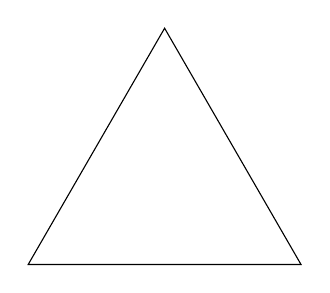
\begin{tikzpicture}
      \node[regular polygon, draw,
        regular polygon sides = 3,
        minimum size = 4cm] (p) at (0,0) {};
    \end{tikzpicture}
  \end{center}

  To keep track of what's going on, put names on your vertices.

  There are only 6 possible symmetries of this group. Symmetries are determined
  by where the labels on the vertices go.
}

Consider an $n$-gon and take $A_1$, any vertex of this $n$-gon. You can take
$A_1$ to any of $n$ vertices, then chose whether to put $A_2$ (a neighbor of
$A_1$) clockwise or counter-clockwise of $A_1$. Then, everything else is determined!

\note {
  $D_{2n}$ is {\bf not} Abelian. Simply convince yourself that rotate then
  reflect is {\it different} from reflect, then rotate. If you're not convinced,
  draw it!
}

\example {
  In $D_{2n}$, if $x$ is a reflection, $y$ is not counter-clockwise by $2 \pi /
  n$ radians
}

{\bf Fact}: $D_{2n} \le S_n$ for $n \ge 3$. Since symmetry in $D_{2n}$ is a
permutation of vertex labels.

{\bf Exercise}: Show that $D_6 \cong S_3$.

\definition {
  If $H \le G$, define

  \[
    aH = \{ ah \mid h \in H \} \subseteq G
  \]

  is called a {\bf left coset} of $H$, with $a \in G$ fixed.
}

{\bf Proposition}: If we have a homomorphism $\phi: G \to G'$, and $a, b \in G$,
then if $K = \ker(\phi)$ (which remember is a subgroup of $G$), then

\[
  \phi(a) = \phi(b) \Leftrightarrow a^{-1}b \in K \Leftrightarrow b \in a K
  \Leftrightarrow a K = b K
\]

What we have is that cosets determine when elements map to the same spot under a
homomorphism.

{\bf Proof}:

$\phi(a) = \phi(b) \Leftrightarrow \phi(a)^{-1}\phi(b) = e \Leftrightarrow
\phi(a^{-1}b) = e \Leftrightarrow a^{-1}b \in K \Leftrightarrow a^{-1}b = k$ for
some $k \in K$, which is true if and only if $b = ak$ for some $k \in K$, again
if and only if $b \in a K$

\begin{align*}
  &\phi(a) = \phi(b) \\
  \Leftrightarrow &\phi(a)^{-1}\phi(b) = e \\
  \Leftrightarrow &\phi(a^{-1}b) = e \\
  \Leftrightarrow &a^{-1}b \in K \\
  \Leftrightarrow &a^{-1}b = k \\
  \Leftrightarrow &ab = k
\end{align*}

\TODO {}

Similarly, $a \in bK$.

\example {
  $a \in bk$ and $b \in ak$ if and only if $aK = bK$.
}

In fact, for any subgroup $H \le G$, $a^{-1}b \in H \Leftrightarrow b \in aH
\Leftrightarrow aH = bH$.

So given $H \le G$, define a relation $\sim$ no $G$ by $a \sim b \Leftrightarrow
a \in bH$. But by the above, this true if and only if $aH \Leftrightarrow bH$.
Hence $\sim$ is an equivalence relation.

What we get out of this is that

\begin{enumerate}
  \item {\bf the cosets of $H$ partition $G$}.
  \item The number of cosets of $H$ is the index of $H \in G$, written $[G : H]$, which may be $\infty$.
\end{enumerate}

\QUESTION {} How do we compute $[G : H]$?

\date{Mon 12 Feb 2024}

\note {
  \begin{itemize}
    \item Homework 3 is due Thursday this week
    \item Midterm 1 is two Fridays from today.

      Exam content will be up until Monday, and there will be a review on
      Wednesday.
  \end{itemize}
}

\section{Cosets}

{\bf Recall}: If $H \le G$, and $a \in G$, the {\it left coset} $aH = \{ah \mid
h \in H \}$.

Last time we saw that $a \in bH$ if and only if $b \in aH$, if and only if $aH =
bH$, which gives us this equivalence relation $a \sim b \Leftrightarrow a \in
bH$, which means we get a partition on the set $G$ of this group, and it's
partitioned on the cosets! So the cosets of $H$ partition $G$.

{\bf Lemma}: The size of any coset is the same as the original size of the
subgroup for any element $a \in G$. In other words, all cosets are the same
size!

{\bf Proof}: We can write a map $f: H \to aH$ where $h \mapsto ah$.

Let's prove that this is bijective.

\begin{itemize}
  \item {\bf Injective}: If $f(h) = f(h')$, then $ah = ah'$, but then because
    this is a group, we can multiply by $a^{-1}$ on both sides and so $h = h'$.

  \item {\bf Surjective}: Given $ah \in aH$, then $f(h) = ah$.
\end{itemize}

So $f$ is a bijection, so $|H| = |aH|$.

\note {
  We only care about this when our sets are finite! In that case, injectivity
  and surjectivity are the same {\bf as long as the domain and codomain are the same
  size!}
}

We finally get to one of the landmars of Group Theory, this is


\section{Lagrange's Theorem}
\Theorem {
  If $H \le G$ and $G$ is finite, then $|H|$ divides $|G|$.
}
{
  The cosets of $H$ partition $G$, and all have the same size. Therefore

  \[
    |G| = \sum_{aH} |aH| = \sum_{[G : H]} = |H| [G : H]
  \]

  Where $aH$ is a left coset of $G$.

  Furthermore, $|H|$ divides $|G|$ and $[G : H] = \frac{|G|}{|H|}$
}

\Corollary {
  If $a \in G$, then $|a|$ divides $|G|$
}
{
  $|a| = |\lr {a}|$ and $\lr {a} \le G$ so we are done by Lagrange's Theorem.
}

\note {
  {\bf The converse is not necessarily true!}
}

\Corollary {
  If $|G| = p$ a prime, then $G$ is cyclic.
}
{
  Take $a \in G$, $a \ne e$, then $|a| \ne 1$ (because its not the identity.)
  But $|a| \mid p$, so in fact $|a| = p$. But $|G| = p$ and $\lr {a} \le G$, and
  $\lr {a} = G$, so $G$ is cyclic.

  In fact, every element in $G$ which is not the identity is a generator of the
  group!
}

\Lemma {
  If $G, G'$ are cyclic groups of order $n$, then $G \cong G'$.
}
{
  We saw that $G \cong \Z_n$, and $G' \cong \Z_n$, and so it follows that $G
  \cong G'$.
}

\Corollary {
  All order $p$ groups, $p$ a prime, are isomorphic.
}
{
  Proof Omitted. It just follows from everything we've seen so far!

  {\bf Up to isomorphism}, there is only one group of order $p$.
}

Let's go back and talk about those left cosets.

{\bf Remark}. We can also define {\bf right cosets}

\[
  Ha = \{ ha \mid h \in H \}
\]

And in fact, everything we proved so far could have worked with right cosets
too!

{\it A priori}, the partitions generated by a left and right coset might be
different.

\definition {
  A subgroup $H \le G$ is a {\bf normal subgroup} if

  \[
    aH = Ha
  \]

  for all $a \in G$. We write $H \trianglelefteq G$.
}

If $\phi: G \to G'$ is a homomorphism, then $K = \ker(\phi)$ is normal. The
claim here is that kernels are normal subgroups.

{\bf Proof}:

Given $a \in G$, $aK = \phi^{-1}(\phi(a)) = \{b \in G \mid \phi(b) =
\phi(a)\}$. Since the inverse function might not exist, we're just looking for
the {\it pre-image} here (Recall the proposition from last week.)

\note {
  We could have redone this proposition with right cosets!

  \[
    aK = Ka
  \]
}

We have lots of normal subgroups because we have lots of Homomorphisms.

\example {
  \begin{itemize}
    \item $\sgn : S_n \to (\{\pm 1\}, \times)$ with

      \[
        \sigma \mapsto \begin{cases}
          1 & \sigma \text{ even} \\
          -1 & \sigma \text{ odd}
        \end{cases}
      \]

    \item $\ker(\sgn) = An$ implies $An \trianglelefteq S_n$.
  \end{itemize}
}

An alternative way to prove that $H \trianglelefteq G$:

$aH = Ha$ if and only if $aHa^{-1} = H$.

\note {
  Warning:

  \begin{itemize}
    \item If $ah \in aH = Ha$, it's {\bf not necessarily the case} that $ah = ha$.

      Remember, the sets are equal, but not necessarily the elements! Instead, $ah =
      h'a$ for some $h' \in H$.

    \item Similarly, $aha^{-1} = h^{-1}$, not necessarily $h$.
  \end{itemize}
}

Normal subgroups are perfectly designed for doing algebra with cosets! $H
\trianglelefteq G$, then

\[
  (aH)(bH) = \{(ah)(bh') \mid h, h' \in H \}
\]

What is this set?, Well

\begin{align*}
  (aH)(bH) &= \{(ah)(bh') \mid h, h' \in H \} \\
           &= \{a \underbrace{(hb)}_{\in Hb = bH} h' \mid h, h' \in H \} \\
           &= \{a (b h'') h' \mid h', h'' \in H \} \\
           &= \{(ab)(h'' h') \mid h', h'' \in H \}
\end{align*}

As $h'$ and $h''$ range over $H$, we get all elements of $H$. So this set is
$(ab)$ times all elements of $H$, so we have

\[
  (aH)(bH) = (ah) H
\]

Alternatively, we may write

\begin{align*}
  aH bH &= a(Hb)H = a(bH)H \\
        &= ab (HH) = abH
\end{align*}

With these cosets, we can form new groups! This multiplication of cosets is a
binary operation on the set of cosets.

In order to simplify notation, let $\bar a = a H$, and we let

\[
  G / H = \{aH \mid a \in G\} = \{\bar a \mid a \in G \}
\]

With binary operation $\bar a \cdot \bar b = \overline{ab}$

{\bf Claim}: $G / H$ is a group, and furthermore, $\pi: G \to G / H$ where $a
\mapsto \bar a$, is a group homomorphism, with $\ker(\pi) = H$.

\definition {
  $G / H$ is called the {\bf quotient group} of $G$ by $H$.
}

{\bf Proof of Claim}:

\begin{itemize}
  \item {\bf Proof of Group}

    \begin{itemize}
      \item {\bf Associativity}: $(\bar a \cdot \bar b) \cdot \bar c = \overline
        {ab} \cdot \bar c = \overline{(ab)c}$. Since $G$ is associative,
        $\overline{(ab)c} = \overline{a(bc)}$ and furthermore, $\bar a \cdot
        \overline{bc} = \bar a (\bar b \cdot \bar c)$.

      \item {\bf Identity}: $\bar e = eH = H$ is the identity.
      \item {\bf Inverses}: $\overline{a^{-1}} \cdot \overline{a} =
        \overline{a^{-1} a} = \overline{e}$. So $\overline{a}^{-1} =
        \overline{a^{-1}}$.
    \end{itemize}

  \item {\bf Group Homomorphism}: $\pi(ab) = \overline{ab} = \bar a \cdot \bar b
    = \pi(a) \pi(b)$

  \item {\bf Kernel}: $\pi(a) = \bar e$ if and only if $aH = eH = H$, if and
    only if $a \in eH = H$. So $H = \ker(\pi)$
\end{itemize}

\date {Wed 14 Feb 2024}

\note {
  Recall: the Exam is next Friday, there are 2 practice Midterms. Not
  necessarily from this class, but they are the right material.

  Also on there is Exam 1 material not on homework. Homework style questions on
  material that we didn't have a Homework on. Quotient Groups, First Isomorphism
  Theorem, ...
}

We are talking about normal subgroups and quotient groups. Let's talk about
normal subgroups some more before getting into examples.

We saw that a subgroup is normal if $aH = Ha$ for all $a \in G$, $H \le G$.

{\bf Claim}: $H$ is normal if and only if $aHa^{-1} = H$ for all $a \in G$.
Why is this the same thing?

{\bf Proof}

$\Rightarrow$

Assume $H$ is normal. Let $a \in G$, then we know that $aH = Ha$ (that's what it
means to be normal.) If we want to show that $aHa^{-1} = H$, we must show that
these two sets are subsets of each other.

If $aha^{-a} \in aHa^{-1}$, then $ah \in aH$, but since $aH = Ha$, there exists
some $h'$ with $ah = h'a$. Hence $aha^{-a} = h'aa^{-1} = h' \in H$. So $aHa^{-1}
\subseteq H$. We wanna prove the other direction now.

If $h \in H$, we want to show that $h \in aHa^{-1}$. We know that $h =
haa^{-1}$, but $ha = ah'$ for some $h'$, so $haa^{-1} = ah'a^{-1}$, so $H
\subseteq aHa^{-1}$.

So $H = aHa^{-1}$.

$\Leftarrow$

Assume $aHa^{-1} = H$ for all $a \in G$. We want to show that $aH = Ha$, let $ah
\in aH$, we know that $aha^{-1} \in H$, which means that there exist some
element of $H$ with $aha^{-1} = h'$, and so $ah = h'a \in Ha$. So $aH \subseteq
Ha$.

The other direction works in the exact same way.

--

\example {
  If $K = \ker(\phi: G \to G')$, then $K \trianglelefteq G$, because if
  $aka^{-1} \in aKa^{-1}$, then

  \[
    \phi(aka^{-1}) = \phi(a) \phi(k) \phi(a)^{-1} = e
  \]

  So $aka^{-1} \in K$, so $aKa^{-1} \le K$.

  In fact, $aKa^{-1}$ is the same size as $K$ is conjugation does not change the
  size, so $aKa^{-1} = K$.
}

Now let's talk about quotient groups.

Let $G = S_n$ and $H = A_n$. We saw last time that $A_n \trianglelefteq S_n$
since $A_n = \ker(\sgn)$. Let's check this explicitly.

Given a permutation $\sigma \in A_n$ and $\tau \in S_n$. We want to show that
$\tau \sigma \tau^{-1} \in A_n$.

Well, $\sigma$ is even. If $\tau$ is odd, then so is $\tau^{-1}$ so $\tau
\sigma \tau^{-1}$ is even. If $\tau$ is even, then so is $\tau^{-1}$, so again
$\tau \sigma \tau^{-1}$, so $\tau \sigma \tau^{-1} \in A_n$.

\sidenote {
  Why is it that $|\sigma| = |\sigma^{-1}|$, with $\sigma \in S_n$? Well, just
  think of

  \[
    \sigma = (a_1 a_2)(a_2 a_3) \cdots (a_{k  - 1} a_k)
  \]

  Then

  \[
    \sigma^{-1} = (a_{k - 1} a_k) \cdots (a_2 a_3)(a_1 a_2)
  \]

  so $|\sigma| = |\sigma^{-1}|$.
}

So $\tau \sigma \tau^{-1} \in A_n$, and $A_n$ is normal.

\section{Quotient Groups}

Assume that $H \trianglelefteq G$. Last time, we defined that

\[
  G / H = \{aH \mid a \in G\} = \{\bar a \mid a \in G \}
\]

With the binary operation $\bar a \cdot \bar b = \overline{ab}$.

\example {
  If $G = S_n$ and $H = A_n$. Since $|S_n| = n!$, $|A_n| = n! / 2$. We know that

  \[
    [S_n : A_n] = \frac{n!}{n! / 2} = 2
  \]

  and so $|S_n / A_n| = 2$ and thus $S_n / A_n \cong \Z_2$. \QUESTION{} Why is this
  isomorphic?
}

{\bf Remark}: ``Identify the quotient group" means ``Find a familiar group to
which the quotient group is isomorphic."

\example {
  Identify $S_n / A_n$. The answer is $S_n / A_n \cong \Z_2$
}

{\bf $S_n / A_n$ in more detail.}

The cosets of $A_n$ are: either

\begin{itemize}
  \item $A_n$ (the coset of even permutations)
  \item $(12)A_n$ (the coset of odd permutations)
\end{itemize}

So $S_n / A_n = \{ \bar e, \overline{(12)} \}$

\TODO{} see multiplication table.

This is clearly isomorphic to $\Z_2$, where we just send $\bar e \to \bar 0$ and
$\overline{(12)} \to \bar 1$.

\example {
  Consider $G = \Z_n$, $H = \lr{\bar m}$ for $\bar m \in \Z_n$.

  {\bf Fact}: Any subgroup of an Abelian group is normal. This should make
  sense, because left and right cosets only different by the order in which you
  write, which doesn't matter for Abelian groups!

  Say that $\gcd(m, n) = d$, then $|\bar m| = \frac{n}{d}$. Take $[G : H] = |G /
  H|$, and we know by Lagrange's theorem that $|G / H| = |G| / |H| = n / (n / d)
  = d$.

  On Homework 2, we showed that if $\phi: G \to G'$ is onto and $G$ is cyclic,
  then $G'$ is cyclic.

  Here, we have the onto homomorphism $\pi: G \to G / H$. Since $G$ is cyclic,
  so is $G / H$, which means $G / H$ is a cyclic group of order $d$, hence $G /
  H \cong \Z_d$.
}

Alternatively: Assume that $\bar m$ is the smallest element in $H$ (i.e. $\bar m
= \bar d$.)

What are the cosets?

The cosets of $H$ are

$\{\bar 0 + H, \bar 1 + H, \dots, \overline{d - 1} + H\}$, and $\bar a + H = H
\Leftrightarrow \bar a \in H$, since $aH = eH \Leftrightarrow a \in eH = H$.

We can already see that $G / H$ is cyclic, generated by $\bar 1 + H$. Hence $G /
H \cong \Z_d$, where $\phi(\bar k + H) = \bar k$.

Our goal is to prove the

\Theorem {
  1st Isomorphism Theorem.
}
{
  If you have a homomorphism $\phi: G \to G'$, then $G / \ker(\phi)$, since
  $\ker(\phi)$ is normal. Furthermore,

  \[
    G / \ker(\phi) \cong \image(\phi)
  \]
}

\example {
  Take $\sgn: S_n \to \Z_2$, but this time with

  \[
    \sigma \to \begin{cases}
      \bar 0 & \sigma \text{ even} \\
      \bar 1 & \sigma \text{ odd} \\
    \end{cases}
  \]

  $\sgn$ is onto, so $\image = \Z_2$. $\ker(\sgn) = A_n$, then $S_n / A_n \cong
  \Z_2$.
}

\example {
  $\phi: \Z \to \Z_n$ with $k \to \bar k$.

  $\phi$ is onto, $\ker \phi = n \Z$, then $\Z / n\Z \cong \Z_n$
}

\date{Fri. 16 Feb 2024}

Let's look at some examples of homs

\example {
  Consider $\det: \gl_n(\R) \to (\R \setminus \{0\}, \times)$. We know that
  $\ker(\det) = \{ A \in \gl_s(\R) \mid \det(A) = 1 \} = \sl_n(\R)$, and we now
  see that this is a normal subgroup.

  $\sl_n(\R) \trianglelefteq \gl_n(\R)$, as given any $A \in \sl_n(\R)$, $B \in
  \gl_n(\R)$, $BAB^{-1}$ has $\det = 1$, so $BAB^{-1} \in \sl_n(\R)$, so
  $\sl_n(\R)$ is normal.
}

Because both of these groups are infinite, and so is the index, we can't just
cheat like last time and take a look at what this is isomorphic to. We also know
that $\det$ is surjective, but the 1st isomorphism theorem tells us that
$\gl_n(\R) / \sl_n(\R) \cong \R \setminus \{0\}$.

One more example before the proof.

\example {
  Consider $\varphi: \C \setminus \{0\} \to \R \setminus \{0\}$ with $\varphi(z)
  = |z|$, the map which takes a complex number to its modulus (its length.)

  {\bf Fact}: $|zw| = |z| |w|$, so $\varphi$ is a homomorphism.

  Notice that that the image of $\varphi$ is only positive numbers, and
  $\ker(\varphi)$ is all the complex numbers with modulus $1$ (or length 1.)
  This is all complex numbers of the form $a + bi = 1$, so $a^2 + b^2 = 1$,
  which is the unit circle!

  Here, our 1st isomorphism theorem tells us that $\C \setminus \{0\} /
  \text{unit circle} \cong \R_{\ge 0}$.

  Think about this:

  \[
    \C \setminus \{0\} = \{re^{i \theta} \mid r \in \R_{\ge -0}, e^{i\theta} \in
    \text{ unit circle}\}
  \]

  What we're left with is just the module information.
}

{\bf Question}: Can you quotient out by the real numbers? Well remember that
complex numbers under multiplication is Abelian, so every subgroup is normal,
which means that you can! Do you get something isomorphic to the unit circle?
Think about it!

Ok! Time for the theorem.

\section{1st Isomorphism Theorem}


\Theorem {
  Given a homomorphism $\varphi: G \to G'$, we have that

  \[
    G / \ker(\varphi) \cong \image(\varphi)
  \]
}
{
  We have a hom $\varphi: G \to G'$. Let's assume that it's onto. If it's not,
  replace $G'$ to $\image(\varphi)$ (Basically, we just change the codomain to
  make it onto.)

  Let $K = \ker(\varphi)$, and we want to show that $G / K \cong G'$. Let $\pi:
  G \to G / K$ (since $K$ is normal, we can do this!) This is the map $\pi(a) =
  \bar a$.

  We define $\bar \varphi: G / K \to G'$, which takes $\bar \varphi(\bar a) =
  \varphi(a)$


  Here's a picture.
  \TODO{}

  % https://q.uiver.app/#q=WzAsMyxbMCwwLCJHIl0sWzIsMCwiRyciXSxbMSwxLCJHL0siXSxbMCwxLCJcXHZhcnBoaSJdLFswLDIsIlxccGkiLDJdLFsyLDEsIlxcYmFyIFxcdmFycGhpIiwyXV0=
% \begin{tikzcd}
% 	G && {G'} \\
% 	& {G/K}
% 	\arrow["\varphi", from=1-1, to=1-3]
% 	\arrow["\pi"', from=1-1, to=2-2]
% 	\arrow["{\bar \varphi}"', from=2-2, to=1-3]
% \end{tikzcd}


  we check that $\bar \varphi$ is well-defined, i.e. if $\bar a = \bar b$, check
  that $\bar \varphi(\bar a) = \bar \varphi(\bar b)$

  \begin{align*}
    \bar a = \bar b &\Leftrightarrow aK = bK \\
                    &\Leftrightarrow \varphi(a) = \varphi(b) \\
                    &\Leftrightarrow \bar \varphi(\bar a) = \bar \varphi(\bar b)
  \end{align*}

  So $\bar \varphi$ is a function.

  {\bf Claim}: $\bar \varphi$ is an isomorphism.

  \begin{itemize}
    \item {\bf Homomorphism}:

      $\bar \varphi(\bar a \cdot \bar b) = \bar \varphi(\overline{ab}) =
      \varphi(ab) = \varphi(a) \varphi(b) = \bar \varphi(\bar a) \bar
      \varphi(\bar b)$.

    \item {\bf One to one}:

      We'll show that $\ker(\bar \varphi) = \{ \bar e \}$ (usefull trick btw, if you have a hom, you only need to check this)

      if $\bar \varphi(\bar a) = e$, then $\varphi(a) = e$, but then $a \in
      \ker(\varphi) = K$, so $\bar a = aK = K = \bar e$.

    \item {\bf Onto}:

      if $b \in G'$, then there exists $a \in G$ with $\varphi(a) = b$
      (remember, since we assumed $\varphi$ to be onto!)

      So we get $\bar \varphi(\bar a) = \varphi(a) = b$.
  \end{itemize}

  Hence $\bar \varphi: G / K \to G'$ is an isomorphism, which concludes the
  proof.
}

\note {
  For the exam, don't worry about being able to prove, this. You should be able
  to {\it use} these techniques. You should be able to use the tools and
  techniques from class.

  The techniques that go into proofs are good to understand though!
}

\TODO{} draw tetrahedron with colors. Oh god

Let $G$ be the group of symmetries of the regular tetrahedron. Symmetry is
determined by what it does to vertices. All permutations of vertices are
possible since all vertices are neighbors. Immediately, we see that

\[
  G \cong S_4
\]

Every symmetry also permutes the colors of the edges.

\[
  \{\text{red}, \text{green}, \text{blue}\}
\]

The group of permutations of this set is isomorphic to $S_3$ of course! Because
we have 3 things in it.

So we get a map $\varphi: S_4 \to S_3$ which takes $\sigma$, a symmetry of the
tetrahedron, to the number of ways to permute the $3$ colors.

We're not going to prove that $\varphi$ is a homomorphism.

Let $C_1 = \text{green}, C_2 = \text{blue}, C_3 = \text{red}$. Then $(12) \in
S_4$ is a reflection of the tetrahedron.

\TODO{} draw this somehow

Another way to think about is is that vertices $3$ and $4$ don't move, but $1$
and $2$ switch.

So $\varphi((12)) = (C_1 C_2)(C_3) \in S_3$. It swaps green and blue and keeps
red fixed.

{\bf Exercise 1}: $\varphi$ is surjective. Every way of permuting the colors is
possible.

{\bf Exercise 2}: $\ker(\varphi) = \{e, (12)(34), (13)(24), (14)(23) \}$. This
is the Klein-4 group!!! Also known as $K_4$.

This is a group of order $4$ which is {\bf not} isomorphic to $\Z_4$, since all
elements of $K_4$ are order $1$ or $2$.

Here, the 1st isomorphism theorem tells us that $S_4 / K_4 \cong S_3$.

{\bf Warning}: $K_4$ and $\Z_4$ are Abelian groups of order $4$. Both have
normal subgroups of order $2$. If $K_4 = \{e, a, b, ab\}$, $H = \{e, a\}$ and
$\{\bar 0, \bar 2\} \le \Z_4$, and $K_4 / H \cong \Z_2$, $H \cong \Z_2$, and
$\Z_4 / H \cong \Z_2$.

Why is this a warning? Because we {\bf cannot} reconstruct the original group
from $H$ and $G / H$.

\note {
  We'll do product groups on Monday, which is testable. The rest will not be.
}

\date{Mon. 19 Feb 2024}

Today we are talking about Product Groups!

\section{Product Groups}

Today we try to build up larger groups from smaller groups.

Let's write out explicitly the binary operations. Let $(G, p), (G', p')$ be two
groups.

The set

\[
  G \times G' = \{(g, g') \mid g \in G, g' \in G' \}
\]

Can be given a binary operation

\[
  (g, g') \cdot (h, h') = (p(g, h), p'(g', h'))
\]

Basically, you do the operations component-wise.

{\bf Claim}: This is a group!

\begin{enumerate}
  \item {\bf Identity}: $(e_G, e_{G'})$
  \item {\bf Inverses}: $(g, g')^{-1} = (g^{-1}, (g')^{-1})$
\end{enumerate}

\definition {
  $G \times G'$ is the {\bf product} of $G$ and $G'$. It's also known as the
  {\bf direct product}.
}

\note {
  $|G \times G'| = |G| \cdot |G'|$
}

From this we can get special Homomorphisms. Quite a few in fact.

% https://q.uiver.app/#q=WzAsNSxbMiwxLCJHIFxcdGltZXMgRyciXSxbNCwwLCJHIl0sWzQsMiwiRyciXSxbMCwwLCJHIl0sWzAsMiwiRyciXSxbMCwxLCJcXHBpX0ciXSxbMCwyLCJcXHBpX3tHJ30iLDJdLFszLDAsIlxcaW90YV97R30iLDJdLFs0LDAsIlxcaW90YV97Ryd9IiwyXV0=
\begin{center}
  \begin{tikzcd}
    G &&&& G \\
    && {G \times G'} \\
    {G'} &&&& {G'}
    \arrow["{\pi_G}", from=2-3, to=1-5]
    \arrow["{\pi_{G'}}"', from=2-3, to=3-5]
    \arrow["{\iota_{G}}"', from=1-1, to=2-3]
    \arrow["{\iota_{G'}}"', from=3-1, to=2-3]
  \end{tikzcd}
\end{center}

All of these are homomorphisms. We say that $\iota_G$ and $\iota_{G'}$ are {\bf
inclusions}, and that $\pi_G$ and $\pi_{G'}$ are {\bf projections}. Let's look
at them in more detail

{\bf Inclusions}
\begin{itemize}
  \item $\iota_G(g) = (g, e)$. We have no other choice here for the second
    element. Think about why.
  \item $\iota_{G'}(g') = (e, g')$
\end{itemize}

{\bf Projections}
\begin{itemize}
  \item $\pi_G(g, g') = g$
  \item $\pi_{G'}(g') = g'$
\end{itemize}

Note that these maps are onto, and in fact $\ker(\pi_G) = \{ (e_{G}, g') \mid g'
\in G' \}$. Similarly, $\ker(\pi_{G'}) = \image(\iota_G)$.

Now using the 1st isomorphism theorem, we know that $G \times G' / G' \cong G$.
This means that $\iota_{G'}(G') \le G \times G'$.

Similarly, $G \times G' / G \cong G$, meaning that $\iota_G(G) \le G \times G'$.

This is fairly inline with how we expect the quotient group to behave.

Let's look at an

\example {
  \[
    \Z_2 \times \Z_3 = \{ (\bar 0, \bar 0), (\bar 1, \bar 0), (\bar 0, \bar 1),
    (\bar 0, \bar 2), (\bar 1, \bar 2) \}
  \]
}

Let's turn our attention to $\lr { (\bar 1, \bar 1) }$. We have that

\[
  \lr { (\bar 1, \bar 1) } = \{ (\bar 0, \bar 0), (\bar 1, \bar 1), (\bar 0, \bar
  2), (\bar 1, \bar 0), (\bar 0, \bar 1), (\bar 1, \bar 2) \}
\]

So in fact $(\bar 1, \bar 1)$ is a generator of $\Z_2 \times \Z_3$. This means
that $\Z_2 \times \Z_6$ is not a new group, it's isomorphic to $\Z_6$ ! In fact,
this is generalizable.

{\bf Proposition}

$\Z_m \times \Z_n \cong \Z_{mn}$ if and only if $\gcd(m, n) = 1$.

{\bf Proof}

All we have to do is figure out when the group on the left is cyclic.

{\bf Lemma}:

The order of $(g, g') \in G \times G'$ is the $\lcm(|g|, |g'|)$.

{\bf Proof of Lemma}

If $\gcd(m, n) = 1$, then the $\lcm(|\bar 1|, |\bar 1|) = \lcm(m, n)$. Moreover,

\[
  \lcm(m, n) = \frac{mn}{\gcd(m, n)}
\]

This means that $(\bar 1, \bar 1)$ generates $\Z_m \times \Z_n$, so it is
cyclic, and so it is isomorphic to $\Z_{mn}$

On the other hand, if $\gcd(m, n) \ne 1$, then for any $(\bar a, \bar b) \in
\Z_m \times \Z_n$, then $|(\bar a, \bar b)| = \lcm(|\bar a|, |\bar b|) \le
\lcm(m, n) < mn$, in which case $\Z_m \times \Z_n$ cannot be cyclic! And so it
is {\bf not} isomorphic to $\Z_{mn}$

For instance, $\Z_2 \times \Z_2 \not\cong \Z_4$.

{\bf Proposition}: There are two groups of order $4$, up to isomorphism.

\[
  \Z_4 \text{ or } \Z_2 \times \Z_2
\]

{\bf Proof}: Let $G$ be a group of order $4$. If $G$ is cyclic, then $G \cong
\Z_4$. If not, then $|a| = 2$ for all non-trivial elements in our group. Pick $a
\in G$, and $b \in G$ with $b \ne e$ and $b \ne a$. Then

\[
  ab \ne \begin{cases}
    e & \text{ as } b \ne a^{-1} = a \\
    a & \text{ as } b \ne e \\
    b & \text{ as } a \ne e
  \end{cases}
\]

So $ab$ is the $4$ element of $G$, and thus $G = \{e, a, b, ab\}$. Then we have
that $\varphi: \Z_2 \times \Z_2 \to G$ with

\begin{itemize}
  \item $(\bar 0, \bar 0) \mapsto e$
  \item $(\bar 1, \bar 0) \mapsto a$
  \item $(\bar 0, \bar 1) \mapsto b$
  \item $(\bar 1, \bar 1) \mapsto ab$
\end{itemize}

Is an isomorphism.

{\bf Structure Theorem for Finitely Generated Abelian Groups}

If $G$ is finitely generated, (i.e. there is a finite set $S \subseteq G$ such
that all elements of $G$ are products of elements of $S$ and their inverses) and
$G$ is Abelian, then

\[
  G \cong \Z \times \cdots \times \Z \times \Z_{m_1} \times \cdots \times \Z_{m_k}
\]

Moreover, if $G$ is finite and Abelian, then

\[
  G \cong \Z_{m_1} \times \cdots \times \Z_{m_k}
\]

\btw {
  This is all the material you need to know for this Exam. From this point
  forward is {\bf not} exam material.
}

\section{Semidirect Product}

Given a group $G$, the set $\Aut(G)$ of {\bf automorphisms} of $G$ (i.e.
isomorphisms $G \to G$) is a group under composition.

\definition {
  Let $G, H$ be groups, $\varphi: H \to \Aut(G)$ be a homomorphism with
  $\varphi(h) = \varphi_h$. Then the group

  \[
    G \times_\varphi H \text{ or } G \rtimes H
  \]

  is called a {\bf semidirect product}, where the elements $(g, h) \in G \times
  H$, but the binary operation

  \[
    (g, h)(g', h') = (g \cdot (\varphi_h(g')), hh')
  \]
}

The set is the same! But the binary operation is different, so we have a new
group structure.

The identity: $(g, h)(e, e) = (g \varphi_h(e), he) = (ge, he) = (g, h)$.
On the other side: $(e, e)(g, h) = (e \varphi_e(g), eh) = (eg, eh) = (g, h)$,
since $\varphi_e = \varphi(e) = e_{\Aut(G)}$ so $\varphi_e(g) = g$.

\example {
  If $\varphi: H \to \Aut(G)$ is the identity, then

  \[
    (g, h)(g', h') = (g \varphi_h(g'), hh') = (gg', hh')
  \]

  So

  \[
    G \times_\varphi H = G \times H
  \]
}

\example {
  Let $G = \Z_n$ and $H = \Z_2$ with $\varphi: \Z_2 \to \Aut(\Z_n)$ with $\bar 0
  \mapsto e$ and $\bar 1 \mapsto f$. $f: \Z_n \to \Z_n$ is determined by $f(\bar
  1)$.

  We need $f \circ f = id$ as $\varphi(\bar 1 + \bar 1) = \varphi(\bar 0) = id$.
  For any $n$, $f = id$ or $f(\bar 1) = \overline{-1} = \overline{(n - 1)}$.

  With the former, $\Z_n \times_\varphi Z_2 \cong \Z_n \times \Z_2$. With the
  latter, $\Z_n \times_\varphi \Z_2 \cong D_{2n}$.
}

\newpage
\date{Wed. 21 Feb 2024}

Today is review!

Structure of the Exam:
\begin{itemize}
  \item 4 Questions
  \item First question is short answer. Similar to the 2019 Midterm
  \item 3 Longer questions, similar to the 2019 midterm.
\end{itemize}

{\bf Exam Questions}

\section{Exam 1 Review}

\subsection{Common Groups and their properties}

Useful for having a repertoire of questions.

\begin{itemize}
  \item $\Z$, $\Z_n$. This is {\bf always} under addition by default, {\bf even
    if $n$ is prime!} These are

    \begin{enumerate}
      \item Cyclic
      \item Abelian
      \item Sometimes infinite? Or order $n$
    \end{enumerate}

    \note {
      All subgroups of cyclic groups are cyclic.
    }

  \item $(\Z_n^\times, \times)$. This is the group of integers relatively prime
    to $n \mod n$ under $\times$. It is

    \begin{enumerate}
      \item Abelian
      \item Not necessarily cyclic, so the order is complicated.
      \item Does not include $\bar 0$.
    \end{enumerate}

  \item $S_n$. The Symmetric group. It is

    \begin{enumerate}
      \item Non-Abelian
      \item Not cyclic
      \item $|S_n| = n!$
    \end{enumerate}

    We have some nice isomorphisms

    \begin{enumerate}
      \item $S_3 \cong D_6$, where $D_6$ is the symmetries of a {\bf triangle}.
      \item $S_2 \cong \Z_2$
    \end{enumerate}

  \item $D_{2n}$. The dyhedral group. The symmetries of a regular $n$-gon. It is

    \begin{enumerate}
      \item Non-Abelian
      \item Not cyclic
      \item Order $2n$
    \end{enumerate}

    And we have that $D_{2n} \le S_n$, but we only have $D_6 \cong S_3$.

    We have a nice notation for this. We say that it is generated by $x$, a
    reflection, and $y$ a rotation.

    \[
      D_{2n} = \{e, x, y, \dots, y^{n - 1}, yx, \dots, y^{n-1}x\}
    \]

    And we have that $yx = y^{-1}x$.

  \item $A_n$. The alternating group. $A_n \le S_n$ with

    \begin{enumerate}
      \item $|A_n| = n! / 2$, subgroup of even permutations.
    \end{enumerate}

  \item $\R, \C$ (under addition), $\R \setminus \{0\}, \C \setminus \{0\}, \Q
    \setminus \{0\}$ (under multiplication)

    These are

    \begin{enumerate}
      \item Infinite
      \item Non-cyclic.
    \end{enumerate}

  \item $\gl_n(\R), \sl_n(\R)$. These are

    \begin{enumerate}
      \item Infinite
      \item Non-Abelian
    \end{enumerate}

    Where the binary operation is Matrix multiplication.

  \item Product Groups $G \times H$ with

    \begin{enumerate}
      \item $|G \times H| = |G| \cdot |H|$.
      \item $|(a, b)| = \lcm(|a|, |b|)$.
    \end{enumerate}

    These groups are Abelian if and only if both $G$ and $H$ are Abelian.

    We saw

    \begin{enumerate}
      \item $\Z_2 \times \Z_2 \not\cong \Z_4$, the Klein-4 Group.
    \end{enumerate}

    We also saw $\Z_m \times \Z_n \cong \Z_{mn}$
\end{itemize}

$Z_2$ Can be written a number of different ways.

\example {
  Groups of order $30$.

  We know that $30 = 3 \cdot 5 \cdot 2$.

  \begin{enumerate}
    \item If we want an Abelian group, we have no choice but to use $\Z_{30}$.
      \TODO{} why?

      What about $\Z_2 \times \Z_3 \times \Z_5$? Well that's isomorphic to
      $\Z_{30}$, since $2, 3$ are coprime, and $6, 5$ are also coprime.

    \item Non-Abelian: $D_{30}$, the symmetries of a regular $15$-gon, or
      $\Z_{3} \times D_{10}$, or $\Z_5 \times D_6$.

      Why are these 3 groups different? Why are they not isomorphic?

      The approach is to think about many different things. Usually the approach
      is to find a property that holds in one group that does not hold in the
      other.

      \begin{itemize}
        \item It could be size. If the sizes don't match, no chance that there
          can be an isomorphism.
        \item Abelian-ness
        \item One of them could be that a group has a normal subgroup of order
          $5$, and the other does not.
        \item This group has an element of order $15$, and the other does not.
      \end{itemize}

      All those things can be used to show that things are not isomorphic.

      In the example above, we know that $D_{30}$ has 15 elements of order 2,
      $D_{10}$ for sure has 5. The claim is that this is all of them. Simply
      notice that

      \[
        |(\bar a, g)| = \lcm(|\bar a|, |g|) = \begin{cases}
          \lcm(1, |g|) = |g| \\
          \lcm(3, |g|) = 3|g|
        \end{cases}
      \]

      The problem is that $3|g|$ is never equal to $2$, so it has to be $|g|$.

      \TODO{} finish. So they cannot be isomorphic.
  \end{enumerate}
}

\begin{itemize}
  \item $\Z_2 \cong (\{\bar 0, \bar 1\}, +) \cong (\{\pm 1\}, \times)$
\end{itemize}

{\bf 2018, 7b}

We have a group of order 40, we want to know all Abelian groups of order 40.

How many ways can we write 40 as a product of cyclic groups which are not
isomorphic?

We know that

\[
  40 = 2 \cdot 2 \cdot 2 \cdot 5
\]

Well, we have
\begin{enumerate}
  \item $\Z_2 \times \Z_2 \times \Z_2 \times \Z_5$
  \item $\Z_2 \times \Z_4 \times \Z_5 \cong \Z_{10} \times \Z_4 \cong \Z_2
    \times \Z_{20}$
  \item $\Z_8 \times Z_5 \cong \Z_{40}$
\end{enumerate}

Recall that we were asked for Abelian groups, so its just a product of cyclic
groups.

{\bf How do we show something is normal?}

There are several ways. Two big ones:

\begin{enumerate}
  \item {\bf By the definition}:

    Show that $aH = Ha$ are the same coset for all $a \in G$.

    If there's not many cosets, this isn't too bad.

  \item {\bf Show that $aHa^{-1} \in H$ for all $a \in G$, and for all $h \in H$}

    This implies that $aHa^{-1} = H$.

    In fact, it's sufficient to show the one direction for all elements. This is
    because we know that we have a bijection between a group and its
    conjugation.

  \item {\bf If $G$ is Abelian}

    Then all your subgroups are normal, so we're done!

    This one is less applicable, but useful!
\end{enumerate}

\example {
  {\bf 2019, number 4}

  If $G$ is a group and $Z(G) = \{a \in G \mid ab = ba \forall b \in G \}$ is
  the center of the group.

  We want to show that $Z(G) \trianglelefteq G$, in order words, that it's a
  normal subgroup.

  {\bf Proof}

  $e \in Z$, so $Z \ne \varnothing$

  {\bf Closure}: If $z, z' \in Z$, then for any $a \in G$, then $zz'a = zaz' =
  azz'$ so $zz' \in Z$. So $Z$ is closed.

  {\bf Inverses}: If $z \in Z$, $a \in G$, $az^{-1} = (za^{-1})^{-1} =
  (a^{-1}z)^{-1} = z^{-1}a$ so $z^{-1} \in Z$.

  {\bf WARNING}: If you aren't told it's a subgroup, you have to show that too!

  {\bf Normal}: To show that it's normal, if $z \in Z, a \in G$ then $aza^{-1} =
  aa^{-1}z = z \in Z$ so $Z \trianglelefteq G$.
}

{\bf What's an example of a Bijection that's not a Homomorphism?}

Here's one

\[
  \varphi: \Z_4 \to \Z_4
\]

where

\begin{itemize}
  \item $\bar 0 \mapsto \bar 1$
  \item $\bar 1 \mapsto \bar 2$
  \item $\bar 2 \mapsto \bar 3$
  \item $\bar 3 \mapsto \bar 0$
\end{itemize}

Here, the identity does not map to the identity. Also

\[
  \varphi(\bar 0 + \bar 1) = \varphi (\bar 1) = \varphi(\bar 2)
\]

But

\[
  \varphi(\bar 0) + \varphi(\bar 1) = \bar 1 + \bar 2 = \bar 3
\]

and $\bar 3 \ne \bar 2$.

{\bf 2018, question 2}

$\sigma = (137)(2465)$, and $\tau = (152)(3647)$, want to find $\sigma \tau^{-1}$

Well, $\tau^{-1} = (125)(3746)$

Then $\sigma \tau^{-1} = (1453)(67)$ \TODO{} Show

How do we write this in terms of transpositions? Well

\[
  = (14)(45)(53)(67)
\]



\end{document}
